\documentclass[twoside,11pt]{homework}
\usepackage{amsmath}
\usepackage{graphicx}
\usepackage{enumerate}
\usepackage{float}
\coursename{COMS 4771 Machine Learning (Spring 2018)} % DON'T CHANGE THIS

\studnamea{Yufei Zhao}    % YOUR NAME GOES HERE
\studmaila{yz3170@columbia.edu}  % YOUR UNI GOES HERE
\studnameb{Minghao Li}
\studmailb{ml4025@columbia.edu}
\studnamec{Zhuoran Xiong}
\studmailc{zx2214@columbia.edu}
\hwNo{1}                   % THE HOMEWORK NUMBER GOES HERE

% Uncomment the next line if you want to use \includegraphics.
%\usepackage{graphicx}

\begin{document}
\maketitle

\section*{Problem 1}
\subsection*{(i)}
$$ \int_{-\infty}^{+\infty} p(x|\theta) \,dx = 1
\Rightarrow c \cdot\int_{0}^{+\infty} x^{2}e^{-\frac{x}{\theta}} \,dx = 1, 
\mbox{where c is a constant}
$$
\begin{eqnarray*}
\int_{0}^{+\infty} x^{2}e^{-\frac{x}{\theta}} \,dx
&=& -\theta\int_{0}^{+\infty} x^{2}\,d(e^{-\frac{x}{\theta}})\\
&=& -\theta\cdot(x^{2}e^{-\frac{x}{\theta}}\big|_{0}^{+\infty} - 2\int_{0}^{+\infty}xe^{-\frac{x}{\theta}} \,dx)\\
&=& -2\theta^{2}\int_0^{+\infty}x\,d(e^{-\frac{x}{\theta}})\\
&=& 2\theta^2\int_0^{+\infty}e^{-\frac{x}{\theta}}\,dx\\
&=& 2\theta^3
\end{eqnarray*}
$$\Rightarrow p(x|\theta) = \begin{cases}
\frac{1}{2\theta^3}x^2e^{-\frac{x}{\theta}} &,x \geqslant 0\\\\
0, &,\mbox{otherwise}
\end{cases}$$
\begin{eqnarray*}
\Rightarrow \theta_{ML} &=& \mathrm{arg}\underset{\theta}{\mathrm{\,max}}
\prod_{i=1}^{n}\frac{1}{2\theta^3}x^2e^{-\frac{x}{\theta}}\\\\
&=& \mathrm{arg}\underset{\theta}{\mathrm{\,max}}
\sum_{i=1}^{n} -3\log\theta-\frac{x}{\theta}
\end{eqnarray*}
By finding the critical point, we get
$$\theta_{ML} = \frac{x_1+x_2+\ldots+x_n}{3n}$$

\subsection*{(ii)}
$$p(x|\theta) = \begin{cases}
\frac{1}{2\theta}\,&,-\theta\leqslant x\leqslant \theta\\\\
0&\mbox{,otherwise}
\end{cases}$$
\begin{eqnarray*}
&&\theta < \underset{i}{\mathrm{\,max}}\big\{ |x_i|\big\} 
\Rightarrow \prod p(x|\theta) = 0\\
&&\theta \geqslant \underset{i}{\mathrm{\,max}}\big\{ |x_i|\big\} 
\Rightarrow \theta_{ML} = \mathrm{arg}\underset{\theta}{\mathrm{\,max}}\frac{1}{2^n\theta^n}\\
&&\Rightarrow \theta_{ML} = \underset{i}{\mathrm{\,max}}\big\{ |x_i|\big\}
\end{eqnarray*}

\subsection*{(iii)}
for Gaussian Distribution ($\mu$ is unknown): $$\mu_{ML} = \frac{1}{n}\sum_i x_i$$
$$\sigma_{ML}^2 = \frac{1}{n}\sum_i (x_i - \mu_{ML})^2$$
\begin{eqnarray*}
\mathbb{E}[\mu_{ML}] &=& \frac{1}{n}\sum_i \mathbb{E}[x_i] = \frac{1}{n}\,n\cdot\mu = \mu\\\\
\mathbb{E}[\sigma_{ML}^2] &=& \frac{1}{n}\sum_i \mathbb{E}[x_i^2]-2\mathbb{E}[\mu_{ML}\cdot\frac{1}{n}\sum_i x_i] + \mathbb{E}[\mu_{ML}^2]\\\\
&=& \mathbb{E}[x^2] - \mathbb{E}[\mu_{ML}^2]\\\\
&=& \sigma^2-\sigma_{\mu_{ML}}^2
\end{eqnarray*}
$$\mbox{in which }\sigma_{\mu_{ML}}^2=\mathbb{D}\big[\frac{1}{n}\sum_i x_i\big]=
\frac{1}{n^2}\sum_i \mathbb{D}[x_i]=\frac{1}{n}\sigma^2$$
$$\mbox{so  } \mathbb{E}[\sigma_{ML}^2]=\frac{n-1}{n}\sigma^2\mbox{  is biased}$$
$$\hat{\sigma^2}=\frac{1}{n-1}\sum_i \big(x_i-\mu_{ML}\big)^2\mbox{  is an unbiased estimation}$$

\subsection*{(iv)}
$$\theta_{ML} = \mathrm{arg}\underset{\theta}{\mathrm{\,max}}\,\mathcal{L}(\theta|x)=\mathrm{arg}\underset{\theta}{\mathrm{\,max\,}}\mathbf{P}(x|\theta)$$

Assume that $$g(\theta)_{ML} = g(\theta^*) \neq g(\theta_{ML})$$\\
then we have $$\mathbf{P}(x|\theta^*)>\mathbf{P}(x|\theta_{ML})$$\\
which is contradictory with $$\theta_{ML}=\mathrm{arg}\underset{\theta}{\mathrm{\,max\,}}\mathbf{P}(x|\theta)$$\\
So $$g(\theta)_{ML} = g(\theta_{ML})$$\\
Let$$\sigma = \sqrt[]{\frac{1}{n-1}\sum_i(x_i-\mu)^2}$$
then$$\sigma_{ML}=g(\mu_{ML}) = \sqrt[]{\frac{1}{n-1}\sum_i(x_i-\mu_{ML})^2}$$
\section*{Problem 2}
\begin{enumerate}[(i)]
\item 
We are using mathematic induction method to prove the affirm.

For the easiest situation, which means $D=1$, there can only be two kinds of input as 1 or 0. So it is very simple when designing the decision tree classifier: only one node  with threshold of 0.5 is needed, let's call it $n_{1}$, and its topology is like below:

\begin{figure}[H]
\centering\includegraphics[width=5cm]{onenodetree.jpg}
\caption{one node decision tree}
\label{fig:one node decision tree}
\end{figure}

By the one-node classification, the input is divided into two parts, 1 or 0. Next we can give the result based on the output.  

Next, suppose we have successfully classified $D = N-1$ dimension input binary data. That is shown in the picture below:

\begin{figure}[H]
\centering\includegraphics[width=10cm]{N-1_nodestree.jpg}
\caption{N-1 dimension decision tree}
\label{fig:N-1 dimension decision tree}
\end{figure}
Some explanation: $0$ beside the node(i) is the number in the $n-1$ bit of the input $N-1$ dimensional binary array. It means that when the last bit is 0, say the whole array can be something like :
$$XX...0=>1 or 0$$
where there's $N-1$ bits in this array. 

Then, for $D=N$, we have the following topology:

\begin{figure}[H]
\centering\includegraphics[width=10cm]{multinodestree.jpg}
\caption{N dimension decision tree}
\label{fig:N dimension decision tree}
\end{figure}

That is to say, for each last bit in $N-1$ dimension array, we only need to add one more bit.  And this one more bit will be classified using the decision tree we have discussed in the first step.  Under this circumstances, we have two cases to discuss.

case 1: even after classification, the last bit 1 or 0 won't affect the result since the number 

$XX...0X =>$ the output of $XX...0$. 

case 2: after the classification, the last bit does affect the outputs. For example:

$XX...01=>$ 1 while $XX...00=>$ 0

The two cases have nothing to do with the demonstration because whichever the case is, we have got the result that the $N$ dimension array can be classified by decision tree, given it works well for $N-1$ dimension tree. 
I empathize the two cases to clarify that there maybe several tree structures in this scenario, it could be a full tree or not corresponding to case 2 and 1, which will help analyze the second question.

Continuing the induction process. Finally, by proving that from $D=1$, to $D=N$, the decision tree can functionally replace the binary tree: by giving a threshold between 0 and 1, $$g(x) = f(x) for all x\in [0,1]^D$$
\item for the maximum decision tree scenario, the binary number needs the last bit to classify between each other. That is to say, 

$XX...0$=>1 while $XX...1$=>0
In this case, the maximum height is D-1 since we need $D-1$ layers nodes to do the classification.

The function g is something like I mentioned in the last paragraph: it needs the last bit to distinguish between each other for the different label.
\end{enumerate}


\section*{Problem 3}

In this problem, we need to prove the optimality in continuous space $\mathcal{Y}$.\\

First we are given the predictor as $f(x):=\bbE [Y|X=x]$, and we also define $Q(g)$ for any predictor $g:\mathcal{X} \to \bbR$ as $Q(g):=\bbE \left[(g(x)-y)^2\right]$. Since the optimal predictor we want has the lowest $Q(g)$, we need to prove that for any $g$, we have $Q(f)\leq Q(g)$.

In order to prove this, we can prove that $Q(g)-Q(f)\ge 0$ for any $g(x)$ and $f(x):=\bbE [Y|X=x]$, we can prove this step by step
\begin{align}
  Q(g)-Q(f)&=\bbE_{x,y} [(g(x)-y)^2]-\bbE_{x,y} [(f(x)-y)^2]
\\
  &=\bbE_{x,y} [(g(x)-f(x)+f(x)-y)^2]-\bbE_{x,y} [(f(x)-y)^2]
\end{align}

we have
\[
\bbE_{x,y} [(g(x)-f(x)+f(x)-y)^2]=\bbE_{x,y} [[g(x)-f(x)]^2+2(f(x)-y)[g(x)-f(x)]]
  +\bbE_{x,y}[(f(x)-y)^2].
\]

So, 
\begin{equation}
  Q(g)-Q(f)=\bbE_{x,y} [[g(x)-f(x)]^2+2(f(x)-y)[g(x)-f(x)].
\end{equation}

According to $\bbP(x,y) =\bbP(y|x)\bbP(x)$, we can write $\bbE_(x,y)$ as$\bbE_(x,y)=\bbE_x[\bbE_y(y|X=x)]$. 
Therefore, we can write it in this way
\begin{equation}
  Q(g)-Q(f)=\bbE_x[\bbE_y [[g(x)-f(x)]^2+2(f(x)-y)[g(x)-f(x)]]|X=x]
\end{equation}

If we can prove for each fixed x we have $\bbE_y [[g(x)-f(x)]^2+2(f(x)-y)[g(x)-f(x)]] \ge 0$, then the expect value of this must greater or equal to zero.
\[
  \bbE_y [[g(x)-f(x)]^2+2(f(x)-y)[(g(x)-f(x)]]=[g(x)-f(x)]^2+2\bbE_y[(f(x)-y)[g(x)-f(x)]]
\]

The first part $[g(x)-f(x)]^2$ must $\ge 0$, so what we need to compute is the value of $\bbE_y[(f(x)-y)[g(x)-f(x)]]$. Here we have $f(x):=\bbE [Y|X=x]$ and $x$ is what ever value we can choose, so $f(x):=\bbE [Y]$. Plug in this into $\bbE_y[(f(x)-y)[g(x)-f(x)]]$ and we can get
\begin{align}
\notag  \bbE_y[(f(x)-y)[g(x)-f(x)]]&=\bbE_y[(\bbE [Y]-y)[g(x)-f(x)]]
\\
\notag  &=[g(x)-f(x)](\bbE [Y]-E_y[y])
\\
\notag  &=[g(x)-f(x)](\bbE [Y]-E[Y])
\\
\notag  &=0
\end{align}

So we prove that $\bbE_y [[g(x)-f(x)]^2+2(f(x)-y)[(g(x)-f(x)]] \ge 0$, therefore $Q(g)-Q(f)$. So $f(x):=\bbE [Y|X=x]$ is the optimal predictor with respect to $Q$ for continuous output space.



\section*{Problem 4}
\begin{enumerate}[(i)]
    \item 
    Firstly, to prove the matrix $M$ is symmetric:

    $$M^{T} = AA^{T} = A^{T}A = M$$

    So $M$ is symmetric.

    Secondly, assign a vector $x \in R^{n*d}$, then using the definition proof of positive semi-definite matrix:
    
    $$x^{T}A^{T}Ax = (Ax)^{T}Ax = ||Ax||^2 \geqslant 0$$
    
    So we know that $M$ is symmetric positive semi-definite.
    
    \item 
    Firstly, when N=1, which is the initial point, 
    $$\beta^{(1)} = \beta^{(0)}+\eta\,A^{T}(b-A\beta^{(0)}) = \eta\,A^{T}b$$
    Secondly, assume that it works well when N=i, that is to say:
    $$\beta^{(i)} = \eta\,\sum_{k=0}^{i-1} (I-\eta\,M)^kv$$
    So next let's calculate when $N = i+1$:
    
    (Considering $\beta^{(k)} := \beta^{(k-1)}+\eta\, A^{T}(b-A\beta^{(k-1)}) $)
    $$ $$
    \begin{eqnarray*}
\beta^{(i+1)}
&=& \beta^{(i)}+\eta\,A^{T}(b-A\beta^{(i)}) \\
&=& \eta\,A^{T}b+(I-\eta\,A^{T}A)\beta^{(i)} \\ 
\end{eqnarray*}
we have already known what the $\beta^{(i)}$ is according to the second step. So we replace $\beta^{(i)}$ with its expression.
\begin{eqnarray*}
\beta^{(i+1)}
&=& \eta\,v+(I-\eta\,A^{T}A)\,\eta\,\sum_{k=0}^{i-1} (I-\eta\,M)^kv \\
&=& \eta\,v+\eta\,\sum_{k=1}^{i} (I-\eta\,M)^kv \\
&=& \eta\,(1-\eta\,M)^0v+\eta\,\sum_{k=1}^{i} (I-\eta\,M)^kv\\
&=& \eta\,\sum_{k=0}^{i} (I-\eta\,M)^kv
\end{eqnarray*}
Meanwhile, when calculating $\beta^{(i+1)}$ using 
$$\beta^{(i+1)} = \eta\,\sum_{k=0}^{i} (I-\eta\,M)^kv$$
we could also get the same result.

Finally, for any given $N=i$, $N=i+1$ works fine. Since the first number 1 is fit, then the expression satisfies any given N.  
    \item To solve this problem, we applied an important property of eigenvalue:
    
    If $\lambda$ is the eigenvalue of matrix $A$, then $f(\lambda)$ is the eigenvalue of $f(A)$. 
    
    Here, 
    $$f(M) = \eta\,\sum_{k=0}^{N-1} (I-\eta\,M)^k$$
    Thus, given any eigenvalue $\lambda_{i}$ of $M$, we can calculate $f(\lambda_{i})$ as below:
    \begin{eqnarray*}
f(\lambda_{i})
&=& \eta\,\sum_{k=0}^{N-1} (1-\eta\,\lambda_{i})^k \\
&=&  \eta\, \frac{(1-\eta\lambda_{i})^N}{\eta\lambda_{i}} \\
&=&  \frac{(1-\eta\lambda_{i})^N}{\lambda_{i}}
\end{eqnarray*}

So the eigenvalue of $f(M)$ is $\frac{(1-\eta\lambda_{i})^N}{\lambda_{i}}$ for $i\in [1,d]$ where $d$ is defined as the number of eigenvalues of $M$.

\item 

\begin{eqnarray*}
||\beta^{(N)}-\hat{\beta}||^2_{2}
&=& ||\eta\,\sum_{k=0}^{N-1} (I-\eta\,M)^kv-\hat{\beta}||^2_{2} \\
\end{eqnarray*}
Considering $v = M\hat{\beta}$
\begin{eqnarray*}
||\beta^{(N)}-\hat{\beta}||^2_{2}
&=& ||\eta\,\sum_{k=0}^{N-1} (I-\eta\,M)^kM\hat{\beta}-\hat{\beta}||^2_{2} \\
&=& ||\eta\,\sum_{k=0}^{N-1} (I-\eta M)^kM-I||^2_{2}\,||\hat{\beta}||^2_{2} \\
&=& ||I-\eta\,\sum_{k=0}^{N-1} (I-\eta M)^kM||^2_{2}\,||\hat{\beta}||^2_{2} \\
&=& 
\end{eqnarray*}

\end{enumerate}



\section*{Problem 5}
\subsection*{(i)}
To fit training data into Multiple Gaussian model and achieve acceptable accuracy and performance, it is necessary to make sure the covariance matrix $\Sigma$ to be invertible. \\
After look into the training data, it is obvious that a large portion of pixels(out of 784) remain zero for all 10000 samples. These features, which mostly located at corners and margins of the images, are not informational and can cause $\Sigma$ to be singular. \\
To get rid of these features, we followed two steps to preproccess the original data: \\
\begin{enumerate}
\item Treat each feature to be independent from others, compute its variance and pick top 200 features with largest variance.
\item For each sample, apply $x_{ij}' = \frac{x_{ij} - \mu_j}{\sigma_j}$ to normalize each feature to a standard Gaussian distribution.
\end{enumerate}
Then, with the preprocessed data(10000$\times$200), we can train the classifier with MLE.
\begin{enumerate}
\item Split 10000 samples into training and test set.
\item Go through all training samples, count number and compute mean vector and covariance matrix for each class.
\item For each test sample, fit it into models of all classes, and predict its class with which maximum $\mathbf{P}(X|Y)\mathbf{P}(Y)$.
\end{enumerate}
\subsection*{(ii)}
To implement a k-NN classifier without k-d tree is pretty simple:
\begin{enumerate}
\item For each test sample, compute distances between it and all training samples. Pick k training samples with smallest distance.
\item Predict the class of test sample with the majority label among the k training samples previously picked.
\end{enumerate}
This naive implementation is quite slow, comparing with the previous classifier. With a split of (9000, 1000) of training and test set, it takes up to 80 seconds to classify all test sample(around 80ms for each sample).
\subsection*{(iii)}
The probabilistic classifier has higher accuracy over k-NN classifier, both on different training size and on different portion of training data. The following two figures shows how accuracy of these two classifier changes in terms of size and portion of training set, perspectively.\\
\begin{figure}[H]
\centering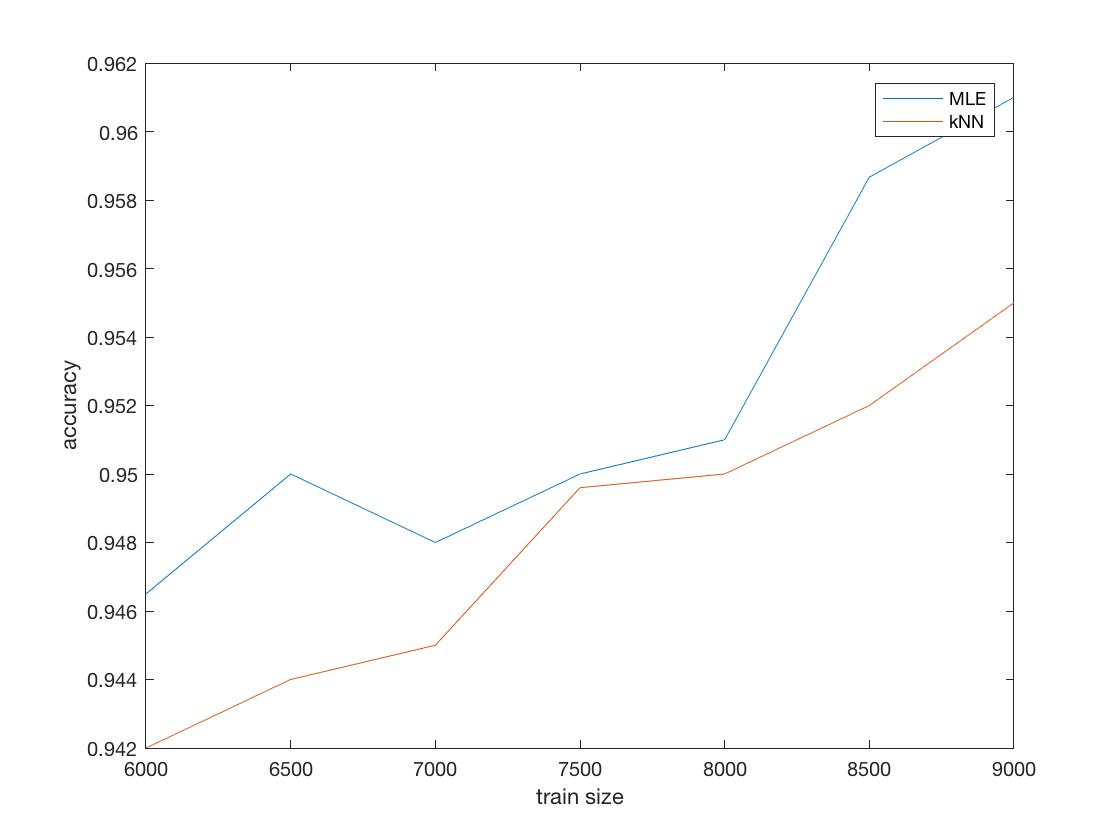
\includegraphics[width=4.8in,height=3.6in]{images/p5_3.jpg}
\caption{accuracy of MLE and kNN with different training size}
\end{figure}
\begin{figure}[H]
\centering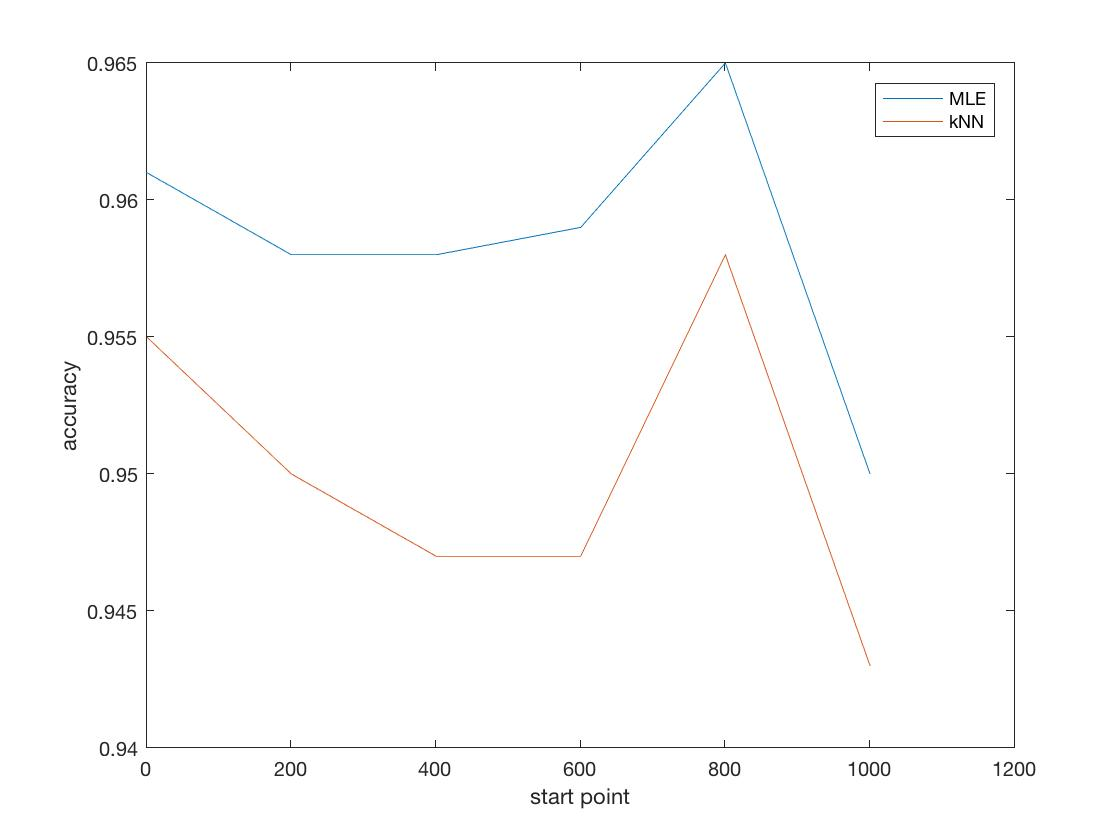
\includegraphics[width=4.8in,height=3.6in]{images/p5_32.jpg}
\caption{accuracy of MLE and kNN with different part of training data}
\end{figure}

From the perspective of speed, the probabilistic classifier is definitely better than k-NN classifier. Because for each test sample, it only computes probability for each class, while k-NN have to go through every training sample to compute their distance(when k-d tree is not implemented).
\subsection*{(iv)}
After testing k-NN with L1, L2 and L$\infty$ on 9000 rows of training data, with k from 1 to 7, it is clear that L1 and L2 have similar performance, which is much better than L$\infty$.\\
\begin{figure}[H]
\centering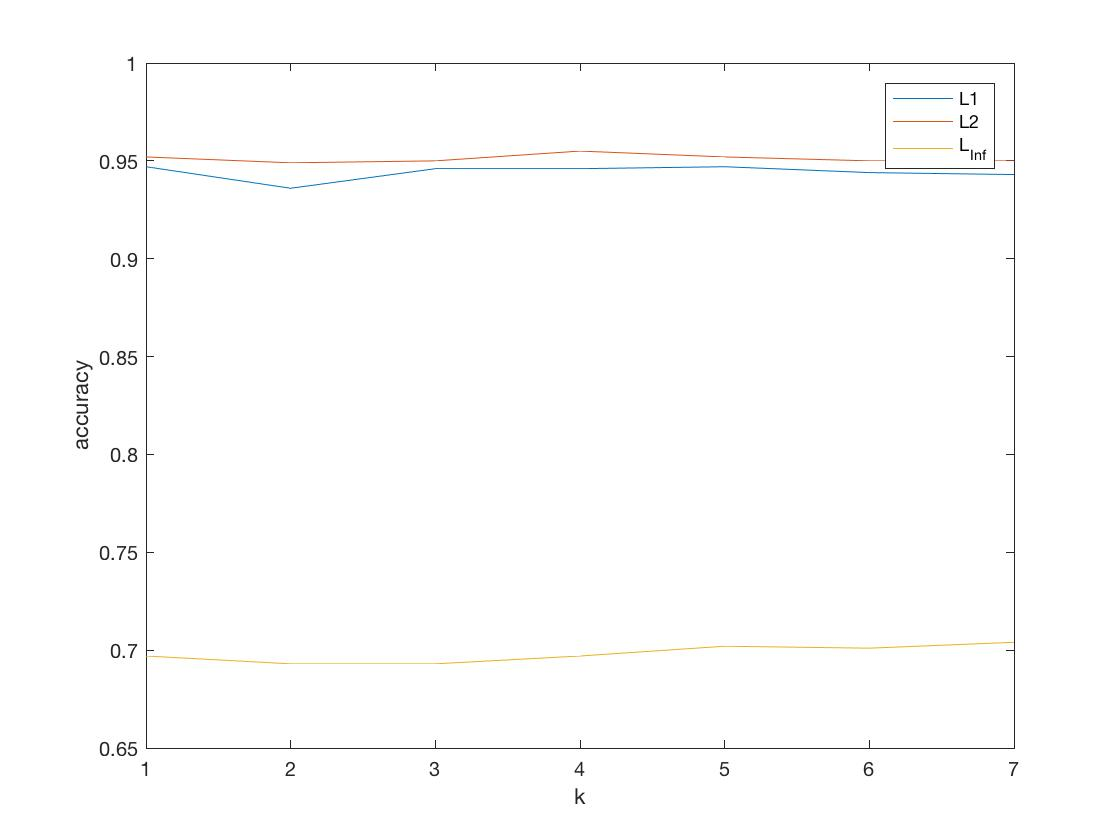
\includegraphics[width=4.8in,height=3.6in]{images/p5_4.jpg}
\caption{accuracy of different distance measurements}
\label{fig:accuracy of different distance measurements}
\end{figure}


\section*{Problem 6}
\subsection*{(i)}
Design procedure:\\
\indent1. Process the data:\\
\indent\indent(a) Load the data from the .mat file. In order to the speed up the data, this program only picks the pixels with the biggest variance;\\
\indent\indent(b) Split the data. First nees to shuffle the data. Then, this program use the idea of stratified split to make sure that the ratio of each classe in training set is the same as the ratio in the test set.\\
\indent2. Write algorithm to evaluate the uncertainty. This program choose to use Gini Index as measurement. This measurement of uncertainty is used to evaluate which kind of splits is better and find the best threshold. \\
\indent3. In the tree algorithm, the tree fist split the whole training set and do it recursively until there is only one data or the depth exceed the maximum depth K.\\
\indent4. According to the decision tree built by the training data, do predict according to the data and get the predict result.\\
\indent5. In the end, compute the error rate of train and test set and plot the line.\\

\subsection*{(ii)}
\begin{figure}[H]
\centering\includegraphics[width=12cm]{images/p7_70_.png}
\caption{Trends of error rate of training set and test set(split rate=0.7)}
\label{fig:Trends of error rate of training set and test set(split rate=0.7)}
\end{figure}

\subsection*{(iii)}
According to the graph, trends of error rate change a little. Because the trends of error 50\% train set and 30\% training set nearly have the same training error rate, just as Figure 7.2 and Figure 7.3 show. However, since we have fewer training data, the final test error is higher when the train set is smaller. 
\begin{figure}[H]
\centering\includegraphics[width=12cm]{images/p7_50_.png}
\caption{Trends of error rate of training set and test set(split rate=0.5)}
\label{fig:Trends of error rate of training set and test set(split rate=0.5)}
\end{figure}
\begin{figure}[H]
\centering\includegraphics[width=12cm]{images/p7_30_.png}
\caption{Trends of error rate of training set and test set(split rate=0.3)}
\label{fig:Trends of error rate of training set and test set(split rate=0.3)}
\end{figure}
	
\subsection*{(iv)}
First, when the K is small, the distribution of the training set can not be easily found with such a shallow tree. So the model is too simple to fit the training dataset. Also, the test dataset is also be hard to fit with this distribution.\\
Then, then the K is growing, the tree have more modes, each nodes can separate the dataset with the best threshold right now. Then the distribution of the training set can be better represent by more complex model.\\
When the model become more complex, the distribution can be perfectly represent by the complex tree. However, this tree is only an representation of distribution of training dataset, the test set will have difference with then training data set, so the test set error will always contain the difference with training data set. \\
When the tree become too complex, which means the depth of the tree is bigger, it can perfectly fit the training set, maybe even one percent fit. Then, some random nose of the training set may also be included in the tree and this can lead to wrong prediction of the test set. Therefore, the test error may sometimes be higher when the depth of the tree become larger.
\subsection*{(v)}
Based on the plot of the trends of testing error, in order to have lower test error rate and higher speed performance, K = 10 is a good setting for the depth of the decision tree when the ration of training data is 70\%. 
\end{document} 





